\documentclass[11pt,compress,t,notes=noshow, aspectratio=169, xcolor=table]{beamer}

% Can only be executed locally, as the 'lecture_iml' submodule is accessed (which is not included in Overleaf). 
% Before executing this script, please ensure that the latest PDF files are available in the 'slides-pdf' folder in 'lecture_iml'.

\usepackage{../../style/lmu-lecture}
\usepackage{pdfpages}
% Defines macros and environments
\input{../../style/common.tex}


\title{Interpretable Machine Learning}
% \author{LMU}
%\institute{\href{https://compstat-lmu.github.io/lecture_iml/}{compstat-lmu.github.io/lecture\_iml}}
\date{}

\begin{document}


%% INTRO


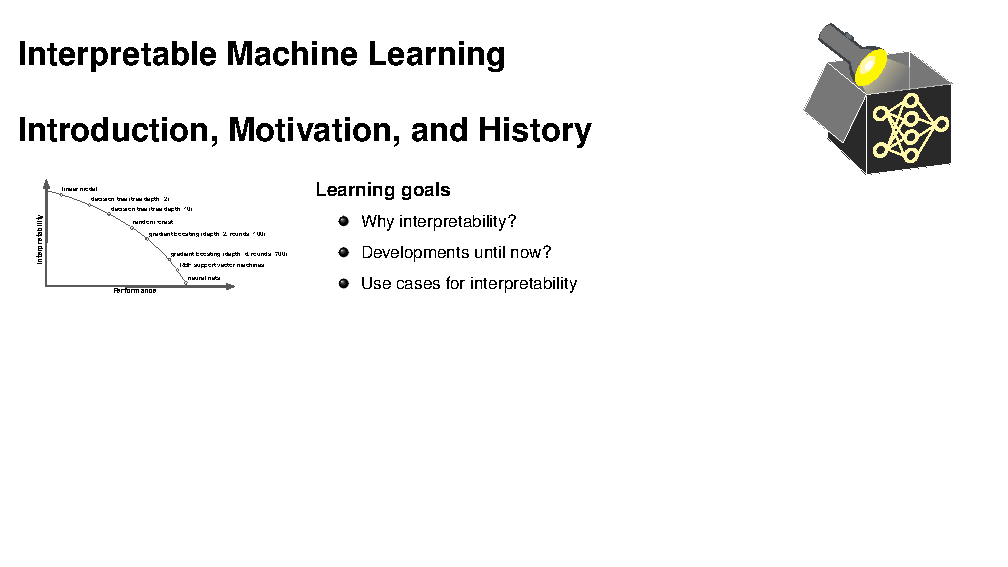
\includepdf[pages={1-6}]{../IML_pdfs_AML/slides01-intro-motivation.pdf}
% 
\includepdf[pages={1}]{../../lecture_iml/slides-pdf/slides01-intro-motivation.pdf}

% 
\includepdf[pages=-]{../../lecture_iml/slides-pdf/slides02-intro-goals.pdf}

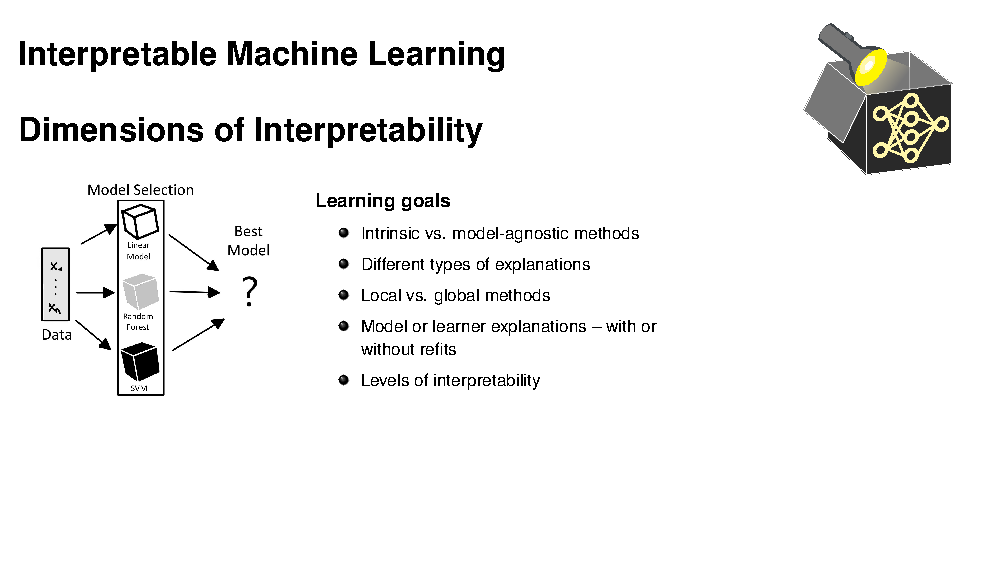
\includepdf[pages={1-13}]{../IML_pdfs_AML/slides03-intro-dimensions.pdf}

%
\includepdf[pages={1-7,16-21}]{../../lecture_iml/slides-pdf/slides01-le-intro.pdf}


%% LIME

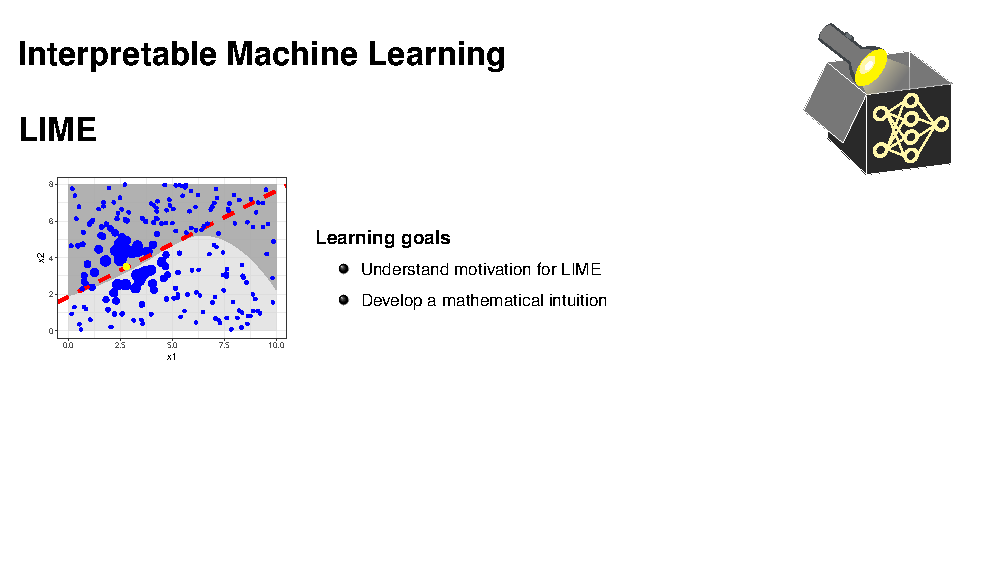
\includepdf[pages=-]{../IML_pdfs_AML/slides04-le-lime.pdf}
\includepdf[pages={2-4}]{../IML_pdfs_AML/slides05-le-lime-example.pdf}
\includepdf[pages={2}]{../IML_pdfs_AML/slides06-le-lime-pitfalls.pdf}


%% Counterfactual Explanations

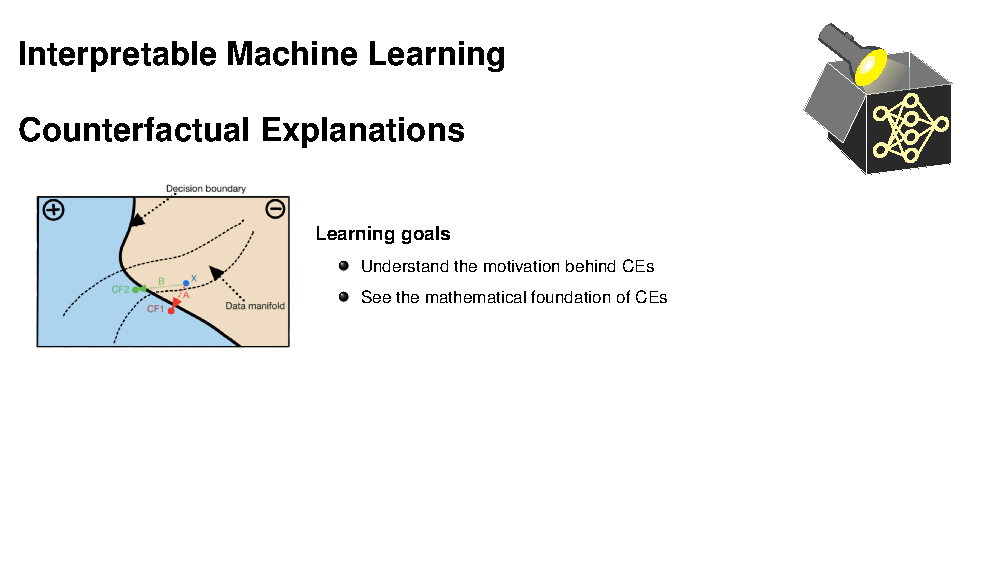
\includepdf[pages={1-8,24-34}]{../IML_pdfs_AML/slides07-le-counterfactuals.pdf}
\includepdf[pages={11-13}]{../IML_pdfs_AML/slides08-le-counterfactuals-methods.pdf}


%% INTRO FE

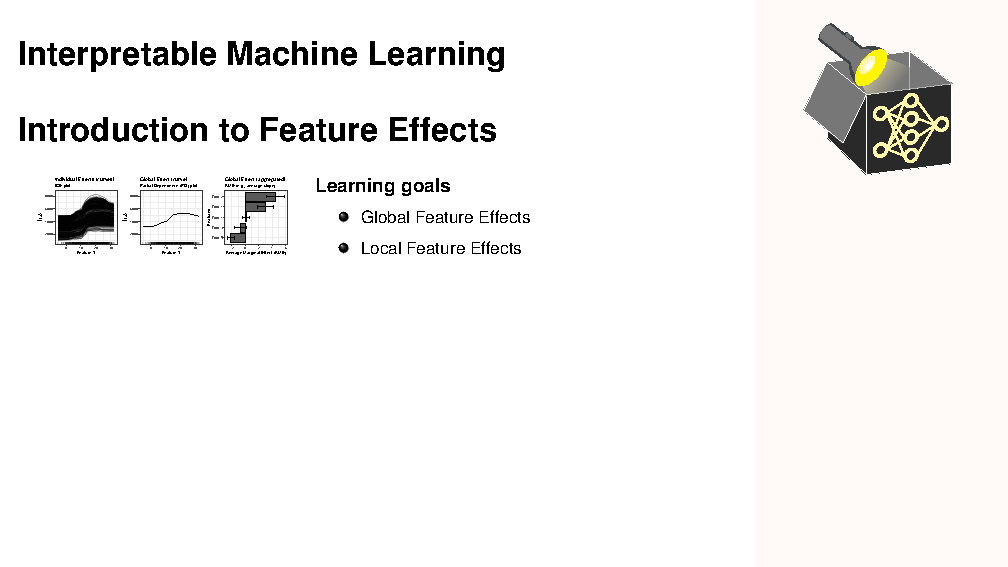
\includepdf[pages=-]{../IML_pdfs_AML/slides01-fe-intro.pdf}


%% ICE Curves

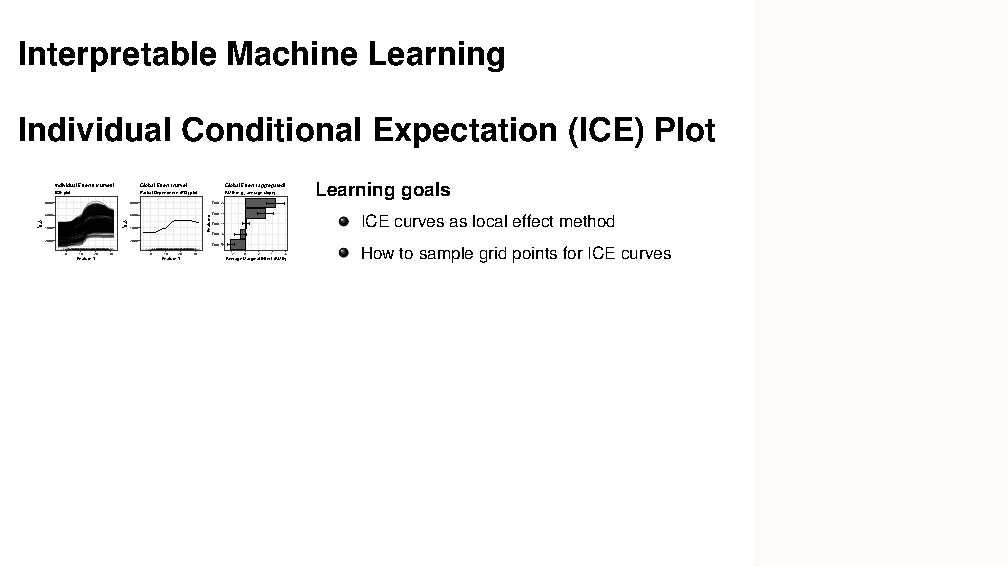
\includepdf[pages={1-10}]{../IML_pdfs_AML/slides02-fe-ice.pdf}


\end{document}